%---------------------------------------------------------------------
%
%                         Project Name:Njust LabReport
%
%---------------------------------------------------------------------
%
%                 created by Qingyun Fang <fqy2017@gmail.com>
%
%                        Last-modified: 2017-6-12
%
%---------------------------------------------------------------------

\documentclass[a4paper,12pt]{report}
\usepackage{ctex}
%\usepackage{xeCJK}
\usepackage{times}
\usepackage{setspace}
\usepackage{fancyhdr}
\usepackage{graphicx}
\usepackage{wrapfig}
\usepackage{array}
\usepackage{fontspec,xunicode,xltxtra}
\usepackage{titlesec}
\usepackage{titletoc}
\usepackage[titletoc]{appendix}
\usepackage[top=30mm,bottom=30mm,left=20mm,right=20mm]{geometry}
\usepackage{cite}
\usepackage{listings}
\usepackage[framed,numbered,autolinebreaks,useliterate]{mcode} % 插入代码
\XeTeXlinebreaklocale "zh"
\XeTeXlinebreakskip = 0pt plus 1pt minus 0.1pt

%---------------------------------------------------------------------
%	页眉页脚设置
%---------------------------------------------------------------------
\fancypagestyle{plain}{
	\pagestyle{fancy}      %改变章节首页页眉
}

\pagestyle{fancy}
\lhead{\kaishu~通信工程实验报告~}
\rhead{\kaishu~913104330115~方青云~}
\cfoot{\thepage}

%---------------------------------------------------------------------
%	章节标题设置
%---------------------------------------------------------------------
\titleformat{\chapter}{\centering\zihao{-1}\heiti}{\chinese{chapter}}{1em}{}
\titlespacing{\chapter}{0pt}{*0}{*6}

%---------------------------------------------------------------------
%	摘要标题设置
%---------------------------------------------------------------------
\renewcommand{\abstractname}{\zihao{-3} 摘\quad 要}

%---------------------------------------------------------------------
%	参考文献设置
%---------------------------------------------------------------------
\renewcommand{\bibname}{\zihao{2}{\hspace{\fill}参\hspace{0.5em}考\hspace{0.5em}文\hspace{0.5em}献\hspace{\fill}}}

%---------------------------------------------------------------------
%	引用文献设置为上标
%---------------------------------------------------------------------
\makeatletter
\def\@cite#1#2{\textsuperscript{[{#1\if@tempswa , #2\fi}]}}
\makeatother

%---------------------------------------------------------------------
%	目录页设置
%---------------------------------------------------------------------
\titlecontents{chapter}[0em]{\songti\zihao{-4}}{\thecontentslabel\ }{}
{\hspace{.5em}\titlerule*[4pt]{$\cdot$}\contentspage}
\titlecontents{section}[2em]{\vspace{0.1\baselineskip}\songti\zihao{-4}}{\thecontentslabel\ }{}
{\hspace{.5em}\titlerule*[4pt]{$\cdot$}\contentspage}
\titlecontents{subsection}[4em]{\vspace{0.1\baselineskip}\songti\zihao{-4}}{\thecontentslabel\ }{}
{\hspace{.5em}\titlerule*[4pt]{$\cdot$}\contentspage}


\begin{document}
%---------------------------------------------------------------------
%	封面设置
%---------------------------------------------------------------------
\begin{titlepage}
	\begin{center}
    
\includegraphics[width=0.3\textwidth]{figure//sf1.png}\\
		
    
\includegraphics[width=0.9\textwidth]{figure//sf.jpg}\\

    \vspace{10mm}

    \textbf{\zihao{2}\kaishu{ 自然语言处理基础实验报告}}\\[3cm]

	\vspace{\fill}
	
\setlength{\extrarowheight}{3mm}
{\songti\zihao{3}	


\begin{tabular}{rl}
	
	{\makebox[4\ccwd][s]{学\qquad 院:}}& ~\kaishu 计算机科学与技术学院\\
	
	{\makebox[4\ccwd][s]{姓\qquad 名:}}& ~\kaishu 胡景雯 \,许韬\,王雪松\,张宁 \\

	{\makebox[4\ccwd][s]{指导老师:}} & ~\kaishu 杨沐昀\\

\end{tabular}
 }\\[2cm]

\vspace{\fill}
\zihao{4}
2018秋季学期\\
\today
	\end{center}	
\end{titlepage}

%---------------------------------------------------------------------
%  摘要页
%---------------------------------------------------------------------
\begin{abstract}
\begin{spacing}{1.5}
	{\zihao{-4}}
    
    通过我们团队成员的学习和不断的尝试,我们完成了这个实验项目,最终在开发集合上的测试结果上最好成绩达到0.5,接下来讲一下我们的思路和具体的实现方法以及在数据集合上的合理性论述.
    
\end{spacing}
\end{abstract}

%---------------------------------------------------------------------
%  目录页
%---------------------------------------------------------------------
\tableofcontents % 生成目录

%---------------------------------------------------------------------
%  实验一
%---------------------------------------------------------------------
\chapter{问题简介}
\setcounter{page}{1}
\begin{spacing}{1.5}
\songti\zihao{-4}

\section{数据集合简介}
数据一共被分成了三个集合,分别是training,develop和测试集合.
集合中的数据格式是一样的,都是问句  $\backslash$t 候选答案句 $\backslash$t 关系标注的形式,关系标注表示回答是否是问句的答案.
我们通过观察数据集合,发现同一个问句往往只有一个回答是正确的.我们也发现了少数意外.不过不妨碍我们得出结论.这个问题像极了小学生做的阅读理解问题:对于一个问题从原文中寻找句子来回答这个问题.

\section{评测工具简介}

使用的评测标准是acc@1,使用老师提供的测试文件进行测试,评测的输入包括模型生成的一个文件,其中每一行表示对应的问题和回答的对应程度.
我们通过观察源代码和手动测试发现,这个输入文件之中,数值的相对大小确定的答句顺序是重要的,数值的绝对值大小对于结果没有影响.
我们将所有回答都标记成1,得到的acc@1值和标记成0是一样的.


\begin{figure}[htbp]
	\centering
	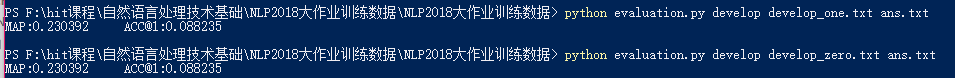
\includegraphics [width=1.0\textwidth]{figure//ceshi.png}
	\caption{测试结果}\label{测试结果}
\end{figure}


\section{问题定义}
我们需要从训练集合和开发集合中训练一个机器学习模型来对测试集合中的数据达到一个比较好的预测效果,能够正确的预测一个问题的多个答案中哪个是相对最正确的.

\end{spacing}



%---------------------------------------------------------------------
%  数据分析
%---------------------------------------------------------------------


\chapter{数据分析}
\setcounter{page}{1}
\begin{spacing}{1.5}
\songti\zihao{-4}

\section{ }
 
\end{spacing}




\chapter{特征提取}
\begin{spacing}{1.5}
\section{特征筛选}

    通过观察问答语句以及相关统计,我们发现,问答语句中的关键词提供了重要的信息,当问答句中存在相同或语义相近的词语时,往往更有可能是能够匹配的问答句。
	故此,通过在查找相关资料,我们采用了两种关键词提取算法。一种是基于tfidf关键词提取技术,另一种为textrank关键词提取技术。两种关键词提取算法都可以对文本进行关键词的提取,并且返回各关键词的权重,使得关键词的利用也有了数据衡量。分别对两种提取的关键词提取4种特征,形成八个特征。四个特征分别为simhash距离,jaccard相似度,关键词交集个数,关键词余弦相似度。
	hashsim为google提出的用于网页文件快速查重的方法。通过哈希函数完成对所有关键词的映射得到hashcode,比较两文本的hashcode汉明距离,即可评判两者相似程度。
	jaccard相似度是一种简单的相似度标准。Set S1,S2,jaccard=$(\#(S1\cap S2))/(\#(S1\cap S2))$
	intersection为集合交集个数。
	关键词余弦相似度cosine:通过计算问答句关键词并集长度,构建文本向量,计算二者文本向量余弦值,即为关键词余弦相似度。
	由于分词技术并不能保证合理的分词,使得关键词的提取未必能在部分问答对中发挥效果。
	我们注意到,在中文中,单个字也能包含部分信息,除关键词外,我们还可以注意问答句中的字的构成。为了衡量问答句的差别,我们提取了问答句的编辑距离作为一个特征,也对该特征做出一定变换实现另一个编辑距离相似度特征,最后还采用了基于文本编辑距离的另一类特征jaro相似度。
	除此以外,近义词的出现在问答句中也占有一定的比例,所以,为了刻画词的相似性,我们采用了相关模型,对语料文本进行了词向量的训练,使得在出现近义词现象,词的相似性得到刻画,提高对问答的匹配度的估计。
	通过统计,问答句的长度之比具有一定分布特性,故此,选取问句长度和答句长度之比作为特征,也可提高预测正确率。

目前提取特征:
\begin{itemize}
  \item tfidf\_hashsim
  \item tfidf\_jaccard
  \item tfidf\_intersect
  \item tfidf\_cosine
  \item textrank\_hashsim
  \item textrank\_jaccard
  \item textrank\_intersect
  \item textrank\_cosine
  \item editdis
  \item editsim: $1 - (float(f\_editdis)/max(len(ques), len(ans)))$
  \item jaro
  \item sentence\_ratio
  \item  word2vec\_sim
\end{itemize}

\end{spacing}





\chapter{解决方案}

\begin{spacing}{1.5}
\section{特征筛选}
	起初,选择特征多达24个,其中还包括了LDA主题模型,LSI主题模型等特征。通过PCA和LDA的降分析,发现其中部分特征几乎不起作用。通过保留和删除的对比实验,也验证了部分特征的无用。最后留下了13个特征。

\section{选取停用词}
	通过简单的试验,我们能够注意到,文本中在分词的过程中会产生大量无明显语义的词,如的,了,呢等,同时,我们还注意到,在问句中,也有一部分问句中的有语义,但无助于特征提取的词,如请问,哪里,什么等。
	我们需要将这部分词语选出作为停用词以提高学习模型的效果。
	通过对问题的单独词频分析,提取问题中的高频词。
	对文本语料按照一问多答进行提取,提取语料中的高频词。
	加上中英文常用标点符号。
	最后人工进行一定的筛选,完成停用词的选择。
\section{选择训练模型}	
    通过对多个模型的简单了解,我们注意到问题尽管是一个分类问题,但是由于数据的严重不平衡,通过猜想和试验,均验证了分类模型的效果不好。
	于是我们采用了回归模型,通过对问答句的相关度进行预测。
	在选取回归模型的时候,我们也有很多的选择。
	由于一些限制,我们选择了xgboost集成模型,就以往经验来看,这个模型在简单机器学习中具有较好表现。不过,我们依旧进行了各种模型的对比,我们选择了基本回归模型如逻辑回归,贝叶斯岭回归,还有SVR,KNN,多层感知机模型和梯度提升回归, XGBoost(eXtreme Gradient Boosting)。
	最后,实验效果显示,xgboost和常规在数据量较大的时候,优于常规gb。



\section{参数调节}

\section{实验分析}

\end{spacing}

%---------------------------------------------------------------------
%  实验感想
%---------------------------------------------------------------------
\titleformat{\chapter}{\centering\zihao{-1}\heiti}{}{1em}{}
\chapter{实验感想}
\begin{spacing}{1.5}
	没什么好说的。
\end{spacing}

%---------------------------------------------------------------------
%  参考文献设置
%---------------------------------------------------------------------
\addcontentsline{toc}{chapter}{参考文献}

\begin{thebibliography}{99}
\songti \zihao{-4} 	
	\bibitem{Leslie.{1994}}
	Leslie Lamport. LATEX: A Document Preparation System.AddisonWesley, Reading, Massachusetts, second edition, 1994, ISBN 0-201-52983-1.
	
	\bibitem{Donald.{1984}}
	Donald E. Knuth. The TEXbook, Volume A of Computers and Typesetting,Addison Wesley, Reading, Massachusetts, second edition, 1984,ISBN 0-201-13448-9.

	
\end{thebibliography}

%---------------------------------------------------------------------
%  附录设置
%---------------------------------------------------------------------
\titleformat{\chapter}{\heiti\Large}{附录~\Alph{chapter}}{11pt}{\Large}
\titlespacing{\chapter}{0pt}{*-4}{*4}

\lstset{breaklines}                %自动将长的代码行换行排版
\lstset{extendedchars=false}
\lstset{language=Matlab}
\renewcommand{\thechapter}{附录\Alph{chapter}.}
\appendix
\begin{appendix}
	
	
\chapter{数据表}
\zihao{-4}\songti
\begin{spacing}{1.5}
	hello world!
\end{spacing}


\chapter{程序代码}
\zihao{-4}\songti
\begin{spacing}{1.5}
下面是一个MATLAB程序的事例,使用了Package mcode,它能较好还原MATLAB本身的编写风格。
\begin{lstlisting}
%The program normalizes the measurement data and compares it to the standard cosine function
data=xlsread('data_sun',1,'B3:E39');
min=[(data(1,1)+data(37,1))/2,(data(1,2)+data(37,2))/2,...
(data(1,3)+data(37,3))/2,(data(1,4)+data(37,4))/2];
max=[data(19,1),data(19,2),data(19,3),data(19,4)];
Min=repmat(min,37,1);
Max=repmat(max,37,1);
data=(data-Min)./(Max-Min);
x=-pi/2:pi/36:pi/2;
y=cos(x);
%----------------------figure-------------------------%
figure(1);
subplot(2,2,1);
plot(x,data(:,1),'ro-');
hold on;
plot(x,y,'b-');
title('R=1.2\Omega');
axis([-2,2,0,1]);
grid on;
subplot(2,2,2);
plot(x,data(:,2),'ro-');
hold on;
plot(x,y,'b-');
title('R=1.6\Omega');
axis([-2,2,0,1]);
grid on;
subplot(2,2,3);
plot(x,data(:,2),'ro-');
hold on;
plot(x,y,'b-');
title('R=2.0\Omega');
axis([-2,2,0,1]);
grid on;
subplot(2,2,4);
plot(x,data(:,4),'ro-');
hold on;
plot(x,y,'b-');
title('R=2.4\Omega');
grid on;
axis([-2,2,0,1]);
\end{lstlisting}
\end{spacing}
\end{appendix}
		

\end{document} 